%----------------------------------------------------------------------------
\chapter{Elméleti bevezetés}\label{ch:elmelet}
%----------------------------------------------------------------------------

Ebben a fejezetben az elméleti háttérről lesz szó. Bemutatásra kerülnek a 3 dimenziós tér alapvető, a diplomamunka során is használt transzformációi, majd pedig az alkalmazott lyukkamera-modell kerül bemutatásra.

%----------------------------------------------------------------------------
\section{A 3 dimenziós tér alapvető transzformációi}
%----------------------------------------------------------------------------

A lineáris algebra legtöbbször egy lineáris transzformációt, egy mátrixszal reprezentál, így egy adott $\mathbf{v}$ vektor $\mathbf{v}'$ transzformáltját a $T$ \textit{transzformációs mátrix}szal való beszorzással kaphatjuk:

\[\mathbf{v}' = T\cdot \mathbf{v}\]

Az affin transzformációkat is hasonlóan leírhatjuk. Például egy $\mathbf{v}(x;\; y)$ vektor $\mathbf{t}(t_x;\; t_y)$ vektorral való eltoltja:

\[\mathbf{v} + \mathbf{t} = (x + t_x;\; y + t_y)\]

A fenti kifejezhető homogén koordinátákkal felírva mátrix-szorzással is:

\[\left[\begin{array}{c}x' \\y'\\ 1 \end{array}\right] = \left[\begin{array}{ccc}1 & 0 & t_x\\0 & 1 & t_y\\ 0 & 0 & 1\end{array}\right] \cdot \left[\begin{array}{c}x \\y\\ 1 \end{array}\right]\]

3 dimenziós vektoroknál ugyanígy alkalmazható, pl. az $x$ tengely körüli $\theta$ forgatás (jobb-kéz szabályt használva):

\[\left[\begin{array}{c}x' \\y' \\z' \\ 1 \end{array}\right] = \left[\begin{array}{cccc}1 & 0 & 0 & 0\\0 & \cos (\theta) & -\sin (\theta) & 0\\ 0 & \sin(\theta) & \cos(\theta) & 0 \\ 0 & 0 & 0 & 1\end{array}\right] \cdot \left[\begin{array}{c}x \\y \\ z\\ 1 \end{array}\right]\]

Gondoljuk meg, hogy ha egy $\mathcal{A}_1, \mathcal{A}_2, \ldots, \mathcal{A}_n$ transzformáció sorozatnak megfelelő transzformációs mátrixok rendre $T_1, T_2, \ldots, T_n$, akkor $v$ transzformáltja:
\[\mathbf{v}' = \mathcal{A}_n(\mathcal{A}_{n-1}(\ldots \mathcal{A}_2(\mathcal{A}_1(\mathbf{v})))\ldots)) = T_n \cdot T_{n-1} \cdot \ldots \cdot T_2 \cdot T_1 \cdot \mathbf{v}\]
Így az eredő transzformációt lényegében úgy kapjuk, hogy a transzformációs mátrixok szorzatával, azaz az ,,eredő transzformációs mátrixszal'' szorozzuk be a vektort:
\[\mathbf{v}' = T \cdot \mathbf{v} \qquad \hbox{ahol} \; T = \prod_{i=1}^{n}{T_i}\]

%----------------------------------------------------------------------------
\section{Lyukkamera-modell \label{sec:pinhole}}
%----------------------------------------------------------------------------

A kamerák a valós világot képezik le egy adott nézőpontból. A lyukkamera-modell alkalmazása során ezt a leképezést, egy perspektivikus projekciónak tekintjük \cite[2.2. fejezet]{pinhole-model} (lásd \aref{fig:pinhole}. ábrát). A projekció középpontját (ahol az egyenesek metszik egymást) \textit{optikai középpontnak} ($C$) vagy \textit{kamera középpontnak}, az egyenest, ami merőleges a képsíkra, és átmegy az optikai középponton \textit{optikai tengelynek}, magát a metszéspontot ($P$) pedig \textit{főpontnak} nevezzük.

\begin{figure}[tbh]
\centering
\tdplotsetmaincoords{60}{130}
\begin{tikzpicture}[line join = round, line cap = round, >=triangle 45, tdplot_main_coords]
  
  \coordinate (O) at (0, 0, 0);
  
  % kocka
  
  \coordinate (C1) at (-4.5, -2, 1);
  \coordinate (C2) at (-4.5, -1, 1);
  \coordinate (C3) at (-4.5, -1, 2);
  \coordinate (C4) at (-4.5, -2, 2);
  \coordinate (C1B) at (-5, -2, 1);
  \coordinate (C2B) at (-5, -1, 1);
  \coordinate (C3B) at (-5, -1, 2);
  \coordinate (C4B) at (-5, -2, 2);
    \node [below right] at (C2) {\small $(X, Y, Z)$};

  \draw [dashed] (C1) -- (C2);
  \draw [dashed] (C2) -- (C3);
  \draw [dashed] (C3) -- (C4);
  \draw [dashed] (C4) -- (C1);
  \draw [dashed] (C1) -- (C1B);
  \draw [dashed] (C2) -- (C2B);
  \draw [dashed] (C3) -- (C3B);
  \draw [dashed] (C4) -- (C4B);
  \draw [dashed] (C1B) -- (C2B);
  \draw [dashed] (C2B) -- (C3B);
  \draw [dashed] (C3B) -- (C4B);
  \draw [dashed] (C4B) -- (C1B);
  
  
  % képsík
  
  \coordinate (I1) at (0, 0, 0);
  \coordinate (I1T) at (-0.5, -0.25, -0.15);
  \coordinate (I2) at (0, 5, 0);
  \coordinate (I2T) at (-0.5, 5.25, -0.15);
  \coordinate (I3) at (0, 5, 3);
  \coordinate (I3T) at (-0.5, 5.25, 3.15);
  \coordinate (I4) at (0, 0, 3);
  \coordinate (I4T) at (-0.5, -0.25, 3.15);
  
  \draw (I1) -- (I2);
  \draw (I2) -- (I3);
  \draw (I3) -- (I4);
  \draw (I4) -- (I1);

  \coordinate (UV) at (0.25, 0.75, 1.25);
  \node [cross] at (UV) {};
  \node [below right] at (UV) {\small $(u, v)$};

  % optikai tengely
  \coordinate (P) at (0, 2.5, 1.5);
  \coordinate (C) at (5, 2.5, 1.5);
  \coordinate (A) at (-1, 2.5, 1.5);

  \node [below] at (C) {\small $C$};
  \draw (C) -- (P);
  \node [cross] at (P) {};
  \node [below right] at (P) {\small $P$};
  \draw [dashed,-latex] (P) -- (A);
  
  % leképezés
  
  \draw [dotted] (C) -- (C2);
  
  % leképezés kerete
  
  \draw [black!15] (C) -- (I1T);
  \draw [black!15] (C) -- (I2T);
  \draw [black!15] (C) -- (I3T);
  \draw [black!15] (C) -- (I4T);
  
\end{tikzpicture}
\caption{Lyukkamera-modell, $(X, Y, Z)$ pont képe a képsíkon $(u, v)$ \label{fig:pinhole}}
\end{figure}

További részletezés nélkül, álljon alább az egyenlet \cite{camera-calib}, amivel egy 3 dimenziós $(X, Y, Z)$ pont 2 dimenziós $(u, v)$ vetületét megkaphatjuk ideális (a kamera nem torzít) esetben:

\[s \left[\begin{array}{c}
u \\ 
v \\
1
\end{array}\right] = \underbrace{\left[\begin{array}{ccc}
f_x & 0 & c_x \\ 
0 & f_y & c_y \\
0 & 0 & 1
\end{array}\right]}_{\mathbf{A}} \left[\begin{array}{ccc|c}
r_{11} & r_{12} & r_{13} & t_1 \\ 
r_{21} & r_{22} & r_{23} & t_2 \\
\undermat{\mathbf{R}}{r_{31} & r_{32} & r_{33}} & t_3 \\
\end{array}\right] \left[\begin{array}{c}
X \\ 
Y \\
Z \\
1
\end{array}\right]\]
ahol:
\begin{itemize}[itemsep=0pt]
\item $s$ a homogén skálázási tényező
\item $\mathbf{A}$ a kamera-mátrix (\textit{belső paraméterek mátrixa})
\item $(c_x, c_y)$ a főpont képsíkbeli koordinátája, amely általában a kép közepe
\item $(f_x, f_y)$ pedig a fókusztávolságok pixelekben kifejezve
\item $\mathbf{R}$ a forgatási mátrix és $\mathbf{t} = \left(\begin{array}{ccc}t_1 & t_2 & t_3\end{array}\right)^T$ az eltolás-vektor -- együttesen $\Big[\,\mathbf{R}\,|\,\mathbf{t}\,\Big]$ a forgatás-eltolás mátrix, mely a \textit{külső paraméterek mátrixa}; azt határozza meg, hogy a statikus világhoz képest a kamera hol helyezkedik el, vagy fordítva, a statikus kamerához a világ hogyan van pozícionálva.
\end{itemize}

\begin{figure}[tbh]
\centering
\begin{subfigure}[b]{.32\linewidth}
	\centering
	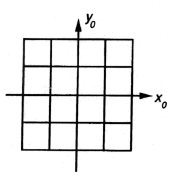
\includegraphics{figures/dist-1.png}
	\caption{Ideális eset}
  \end{subfigure}
\begin{subfigure}[b]{.32\linewidth}
	\centering
	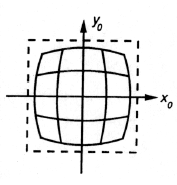
\includegraphics{figures/dist-2.png}
	\caption{,,Hordó-torzítás''}
  \end{subfigure}
\begin{subfigure}[b]{.32\linewidth}
	\centering
	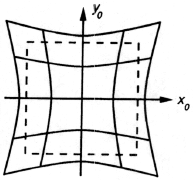
\includegraphics{figures/dist-3.png}
	\caption{,,Tűpárna-torzítás''}
  \end{subfigure}
\caption{Lencsék radiális torzítása \cite{distortion} \label{fig:radial-distortion}}
\end{figure}

Valódi kamerák használata esetén viszont számolnunk kell azzal, hogy a lencséknek van radiális (lásd \aref{fig:radial-distortion}. ábra) és tangenciális torzításuk (ami abból adódik, hogy a lencse és a képalkotó sík nem párhuzamos). Mivel ezek csak a konkrét kamerától függnek, ezért kalibrációval korrigálhatóak, megszüntethetőek. A radiális torzítás esetén:
\[x_{\hbox{\small jav}} = x(1 + k_1r^2 + k_2r^4 + k_3r^6)\]
\[y_{\hbox{\small jav}} = y(1 + k_1r^2 + k_2r^4 + k_3r^6)\]
ahol $(x,y)$ volt az eredeti kép egy pixelének koordinátája, és $(x_{\hbox{\small jav}}, y_{\hbox{\small jav}})$ pedig az új koordináta a korrigált képen. Tangenciális torzítás javítása pedig:
\[x_{\hbox{\small jav}} = x + \Big(2p_1xy + p_2(r^2+2x^2)\Big)\]
\[y_{\hbox{\small jav}} = y + \Big(p_1(r^2+2y^2) + 2p_2xy\Big)\]
Ekkor $k_1, k_2$ és $k_3$ a radiális, $p_1$ és $p_2$ pedig a tangenciális torzítás együtthatói. Magasabb rendű együtthatók is vannak, de ezekkel általában már nem számolunk.
